\documentclass[10pt]{article}
\usepackage[margin=2.2cm]{geometry}\usepackage{graphicx,booktabs,amsmath,url}
\title{Paper-MSM study: smoothed multiscale sampler versus global pCN\\\large Preliminary report}
\author{}\date{5 November 2026}
\begin{document}\maketitle
\section*{Summary}
\begin{itemize}
\item \textbf{The control is reproduced.} E0 (global pCN, all 20 thetas) gives the same posterior as arm 1 of the grid study at $16\times16$ (Gaussian KL $\approx0$, log-$k$ mean field differs by 0.007 rms).
\item \textbf{Mixing.} Every experiment reaches MPSRF $<1.2$. All-at-once runs (E0, E2, E3, E5) do so after 17--22k iterations; coordinate-at-a-time runs (E1, E4, E6) need 89--108k. Updating one \emph{subdomain} at a time (E7, five coefficients) converges after 21k, as fast as all-at-once.
\item \textbf{The MSM posteriors differ from the control.} All six MSM variants are under-dispersed (posterior sd of $\log k$ 0.73--0.81 of the control) and have a larger error against the truth (rms 0.54--0.63 versus 0.42). The paper's smoothing does not repair this; it makes it worse.
\item \textbf{The prior test explains it.} With the likelihood off, projection and smoothing leave the interface band with variance 0.61--0.68 (target 0.97) and weaken the correlation across interfaces (target 0.956): raw 0.00, projected 0.88, smooth-all 0.79, smooth-one/subdomain 0.52--0.59. For E6/E7 this value depends on the step size, i.e.\ the stored-neighbour smoothing makes the prior state dependent. E6 and E7 behave alike, so the lag, not the update unit, is what matters.
\end{itemize}
\section{Setup}
Problem and data as in arm 1 of the grid study ($16\times16$ grid, squared-exponential kernel, correlation length 0.2, 20 global KLE modes, relative-error likelihood $\varepsilon=0.003$, 128 observations, truth from seed 2026). Partition $2\times2$, 5 local modes per subdomain ($p=20$; the tied local pair 5/6 is split, reproducibly by the canonical basis). Smoothing: plain average over a disc of radius $0.1$ within $0.1$ of an interface (112 of 256 cells), no variance inflation. E6/E7 average the band from the new raw field of the moving subdomain and the stored values of the others. The paper's coarse-scale filter is not included. 64 chains per experiment; 100k iterations (adaptation 10k) all-at-once, 150k (adaptation 30k) one-at-a-time; step size adapted to 25\% acceptance, then frozen. Design details: \path|docs/paper_msm_experiment.md|.

\paragraph{How MPSRF/PSRF are computed.} Chains of 64, states saved every 50 iterations; window from iteration 1000 (adaptation included) growing to the end of the run, every second saved sample, curve evaluated every 15 saved samples; $W$ with divisor $n-1$, $B/n$ with divisor $m-1$; MPSRF is the multivariate statistic, PSRF the maximum over coordinates; convergence is the first point (after the first 10) below 1.2; not split-chain. Dimension 20, on the \emph{common coordinates} $z$ (L2 projection of the field onto the 20 global modes) so all experiments are comparable. On the sampler's native state the values agree to the third decimal (e.g.\ E4 1.135, E6 1.101, E7 1.033).

\section{Results}
\begin{table}[h]\centering\footnotesize
\begin{tabular}{lcccccccccc}\toprule
 & acc. & group acc. & iter.\ $<1.2$ & MPSRF & PSRF & sd $z$ & sd $\log k$ & $\Delta$mean & KL & s/chain\\
 &  & range &  & end & end & mean & ratio & $\log k$ & to ctrl &\\\midrule
E0 global, all & 0.252 & 0.25--0.25 & 22k & 1.045 & 1.038 & 0.54 & 1.01 & 0.01 & -0.0 & 22\\
E1 global, one & 0.299 & 0.25--0.44 & 89k & 1.126 & 1.123 & 0.55 & 1.01 & 0.03 & 0.0 & 39\\
E2 raw, all & 0.265 & 0.26--0.26 & 17k & 1.026 & 1.022 & 0.42 & 0.78 & 0.19 & 20.8 & 23\\
E3 proj, all & 0.249 & 0.25--0.25 & 18k & 1.037 & 1.028 & 0.46 & 0.81 & 0.18 & 18.6 & 25\\
E4 proj, one & 0.311 & 0.25--0.51 & 108k & 1.135 & 1.128 & 0.46 & 0.81 & 0.18 & 18.7 & 35\\
E5 smooth, all & 0.255 & 0.25--0.25 & 18k & 1.032 & 1.026 & 0.42 & 0.78 & 0.17 & 19.7 & 26\\
E6 smooth, one & 0.350 & 0.24--0.80 & 89k & 1.101 & 1.087 & 0.41 & 0.73 & 0.25 & 6.0 & 36\\
E7 smooth, subdomain & 0.255 & 0.25--0.26 & 21k & 1.033 & 1.031 & 0.41 & 0.75 & 0.25 & 5.8 & 37\\\\\bottomrule\end{tabular}
\caption{Acceptance after adaptation, convergence, and posterior comparison with the control (arm 1, $16\times16$). sd ratio: mean posterior sd of $\log k$ over the control's; $\Delta$mean: rms difference of the posterior mean $\log k$ from the control's; KL: Gaussian-approximation KL$(\text{MSM}\Vert\text{control})$ of $z$ (large values for E2--E5 because the $z$ covariance is numerically singular, see text).}\end{table}
\paragraph{Acceptance.} All runs adapt to about 25\% overall (0.249--0.255 for all-at-once, E7). In the one-coefficient runs the groups spread: E1 0.25--0.44, E4 0.25--0.51, E6 0.25--0.80, and for some groups in E4 and E6 the adapted step reaches the 0.95 cap (median final step 0.95 for two groups of E6): those coefficients are barely constrained by the data, so they accept almost anything.

\paragraph{Mixing.} See the table: one-at-a-time updates cost about five times more iterations, and E1/E4 end at MPSRF 1.13, close to the threshold. Per-iteration cost is similar (22--39\,s per chain), so all-at-once and E7 are clearly cheapest.

\paragraph{Posterior.} The $z$ covariance for E2--E5 has smallest eigenvalue $\sim10^{-17}$: since $z$ is a linear image of 20 local coefficients, these samplers do not reach all directions of the global span. E6/E7 are not singular (smallest eigenvalue $2\times10^{-4}$) because the stored-neighbour smoothing leaves the span. Posterior sd of $\log k$ is 0.78--0.81 of the control for E2--E5 and 0.73--0.75 for E6/E7, in both band and interior (band/interior 0.70--0.78 / 0.76--0.84). Posterior-mean $\log k$ moves 0.17--0.19 (E2--E5) and 0.25 (E6/E7) rms from the control; the error against the truth rises from 0.42 to 0.54--0.55 (E2--E5) and 0.63 (E6/E7). The pressure field sd is essentially unchanged (ratio 0.99--1.06).

\begin{figure}[h]\centering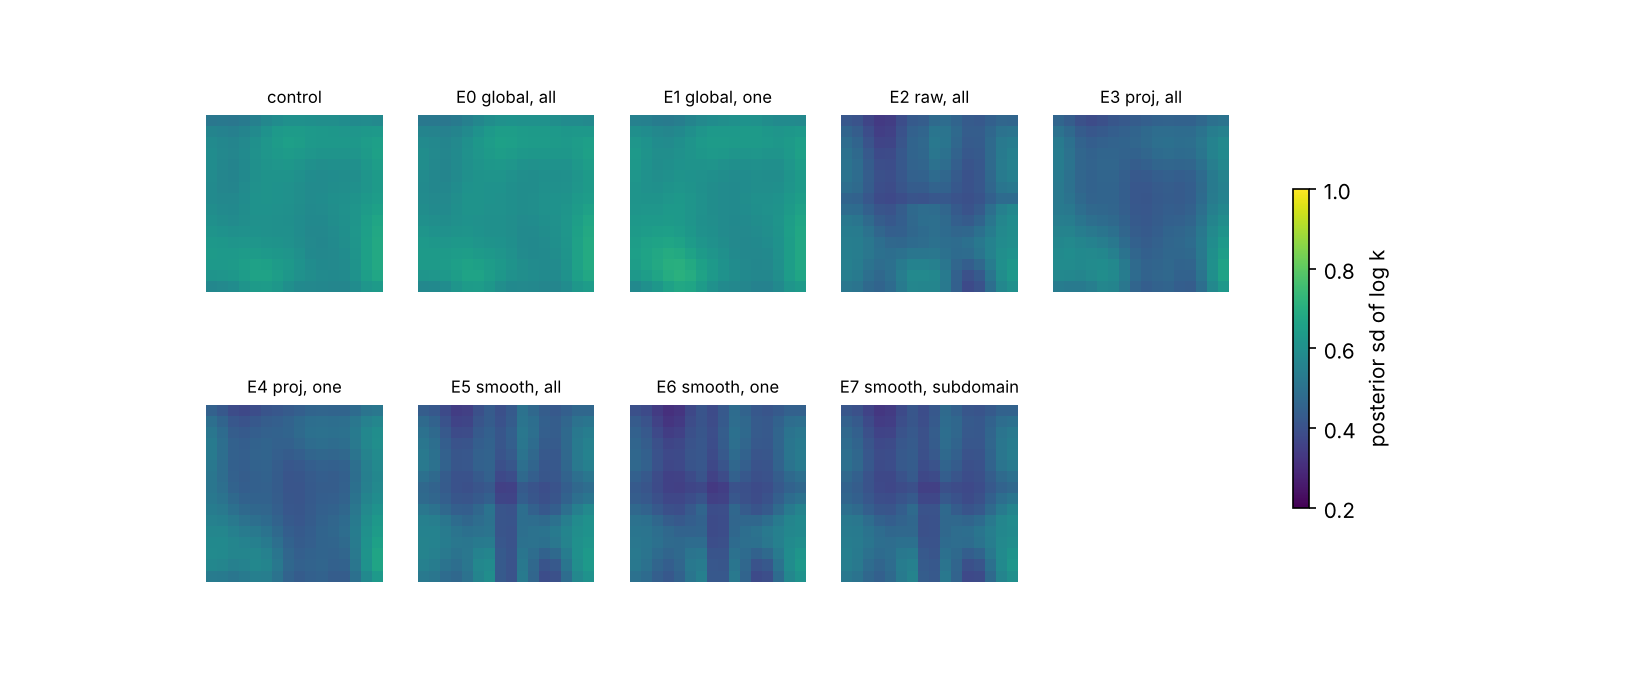
\includegraphics[width=.95\textwidth]{../compare/fig_logk_sd.png}\caption{Posterior sd of $\log k$.}\end{figure}
\begin{figure}[h]\centering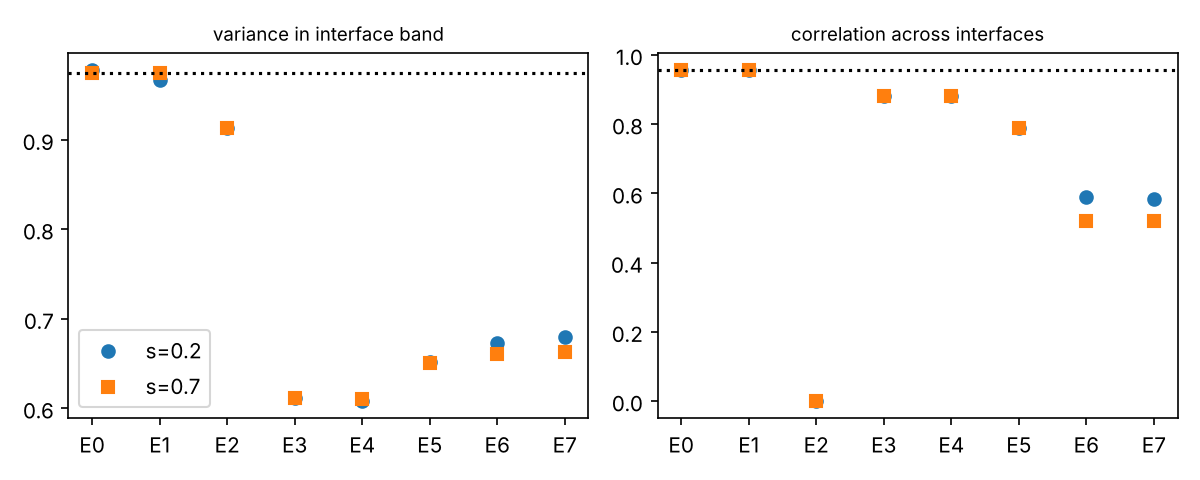
\includegraphics[width=.8\textwidth]{../compare/fig_prior.png}\caption{Prior test (likelihood off), step sizes 0.2 and 0.7; dotted: target prior. Left: mean variance in the interface band. Right: mean correlation of cell pairs facing each other across the interfaces.}\end{figure}

\section{Reading and caveats}
Projection (E3) already costs most of the damage: band variance 0.61 and cross-interface correlation 0.88. The smoothing lowers the correlation further (0.79 all-at-once, 0.52--0.59 with stored neighbours) and does not restore the band variance, so on this problem the smoothing is not an improvement over projection; the old projected MSM and the paper's smoothing are both biased relative to the global prior. The state dependence in E6/E7 (cross correlation 0.59 at $s=0.2$, 0.52 at $s=0.7$) means their stationary prior depends on the adapted step.

Caveats: a single data set and truth; the Gaussian KL is degenerate for E2--E5 and should not be over-read (use the field comparisons); the mechanism is inferred from the prior test, not isolated by a separate experiment; no coarse-scale filter or variance correction was tried.

\paragraph{Sources.} Runs in \path|runs/paper_msm_2026-11/| (\path|compare/table.json|, \path|prior_test/prior_summary.json|); control \path|runs/grid_arms_2026-11/arm1_check_n16|; J.~Comput.\ Phys.\ 497 (2024) 112609.
\end{document}
